% Author: Izaak Neutelings (May 2020)
% Inspiration: https://tex.stackexchange.com/questions/285578/how-to-draw-parallelepiped-and-cube-with-latex/288101#288101
\documentclass[border=3pt,tikz]{standalone}
\usetikzlibrary{arrows,arrows.meta}
\usetikzlibrary{calc}
\usetikzlibrary{decorations.markings}
\usetikzlibrary{angles,quotes} % for pic (angle labels)
\usetikzlibrary{fadings}
\tikzset{>=latex} % for LaTeX arrow head
\usetikzlibrary{3d}

\colorlet{myblue}{blue!80!black}
\colorlet{mypurple}{blue!60!red!90!black}
\colorlet{myred}{red!70!black}
\colorlet{Ecol}{orange!90!black}
\tikzstyle{myarr}=[-{Latex[length=3,width=2]}]
\tikzstyle{Evec}=[Ecol,{Latex[length=2.8,width=2.5]}-{Latex[length=2.8,width=2.5]},line width=1]
\tikzset{
  light beam/.style n args={2}{line width=#2,myblue,line cap=round,decoration={markings,
                     mark=at position #1 with {\arrow{latex}}},
                     postaction={decorate}},
  light beam/.default={0.5}{1}
}
\tikzfading[name=fade out, 
    inner color=transparent!20,
    outer color=transparent!100]
\tikzfading[name=strong fade out, 
    inner color=transparent!0,
    outer color=transparent!99]
\tikzfading[name=atmosphere, 
    inner color=white,
    outer color=black]

\newcommand\molecule[2]{
  \node[ball color=red,circle,inner sep=#2] at (#1) {};
  \node[very thin,draw=red!30!black,fill=red!60!black!70,circle,inner sep=#2,fill opacity=0.3] at (#1) {};
  %\draw[ball color=red,canvas is zy plane at x=0] (0,0) circle(0.5);
}

\newcommand\rightAngle[4]{
  \pgfmathanglebetweenpoints{\pgfpointanchor{#2}{center}}{\pgfpointanchor{#3}{center}}
  \coordinate (tmpRA) at ($(#2)+(\pgfmathresult+45:#4)$);
  \draw[white,line width=0.5] ($(#2)!(tmpRA)!(#1)$) -- (tmpRA) -- ($(#2)!(tmpRA)!(#3)$);
  \draw[mypurple!70!black,line width=0.4] ($(#2)!(tmpRA)!(#1)$) -- (tmpRA) -- ($(#2)!(tmpRA)!(#3)$);
}


\begin{document}


% POLARIZATION by scattering
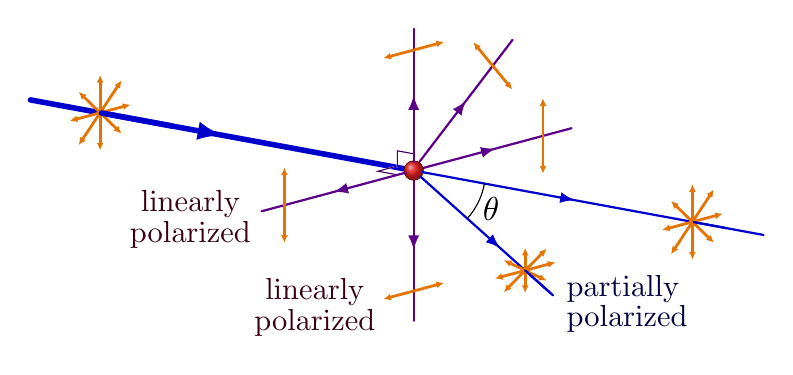
\begin{tikzpicture}[x=(15:0.5), y=(90:0.6), z=(-20:1.3)]
  \def\A{1.0} % initial amplitude
  \def\a{0.8} % scattered amplitude
  \def\L{15}  % length beam
  \def\W{4}   % width horizontal scattered beam
  \def\H{3}   % length horizontal scattered beam
  \def\t{0.8} % thickness scattered beams
  \coordinate (O) at (0,0,0);         % start point
  \coordinate (A) at (0,0,0.10*\L);   % polarization before
  \coordinate (M) at (0,0,0.55*\L);   % molecule
  \coordinate (B) at (0,0,0.95*\L);   % polarization after
  \coordinate (D) at (0,-0.7*\H,0.75*\L); % end point scattered down
  \coordinate (C) at ($(M)!0.8!(D)$); % polarization on MD
  \coordinate (L) at ($(M)+(-\W,0)$); % left scattering
  \coordinate (T) at ($(M)+(0,\H)$);  % top scattered
  \coordinate (Z) at (0,0,\L);        % end point
  
  % BEAMS behind
  \draw[light beam={0.5}{2.0}] (O) -- (M);
  \begin{scope}[canvas is xz plane at y=0]
    \rightAngle{O}{M}{L}{0.6}
  \end{scope}
  \begin{scope}[canvas is zy plane at x=0]
    \rightAngle{O}{M}{T}{0.5}
  \end{scope}
  \draw[light beam={0.5}{\t},mypurple] (M)++(0.01*\L,0) --++ (\W,0);  % scattered right
  \draw[light beam={0.5}{\t},mypurple] (M)++(0,-0.012*\L) --++ (0,-\H); % scattered down
  \draw[light beam={0.5}{\t},mypurple] (M)++(0.01*\L,0.01*\L) --++ (40:0.8*\W) coordinate (TR); % scattered up right
  
  % MOLECULE
  \molecule{M}{2.5}
  
  % BEAMS in front
  \draw[light beam={0.5}{\t}] (M)++(0,0,0.012*\L) -- (Z); % scattered foreward
  \draw[light beam={0.5}{\t},mypurple] (M)++(-0.014*\L,0) -- (L); % scattered left
  \draw[light beam={0.5}{\t},mypurple] (M)++(0,0.012*\L) -- (T); % scattered up
  \draw[light beam={0.6}{\t}] ($(M)!0.05!(D)$) -- (D); % scattered foreward down
  
  % POLARIZATION
  \foreach \ang in {0,45,90,135}{
    \draw[Evec] (A)++(\ang:\a) --++ (\ang-180:2*\a); % before
    \draw[Evec] (B)++(\ang:\a) --++ (\ang-180:2*\a); % after
    \draw[Evec] (C)++(\ang:{\a} and {0.6*\a}) --++ (\ang-180:{2*\a} and {1.2*\a}); % foreward down
  }
  \draw[line width=2.0,myblue,line cap=round] (A)++(0,0,0.002*\L) --++ (0,0,0.1*\L); % overlap
  \draw[line width=\t,myblue,line cap=round] (B)++(0,0,0.002*\L) --++ (0,0,0.1*\L); % overlap
  \draw[line width=\t,myblue,line cap=round] ($(C)!0.001!(D)$) -- ($(C)!0.9!(D)$); % overlap
  \draw[Evec] (M)++(-\a, 0.85*\H) --++ (2*\a,0); % top
  \draw[Evec] (M)++(-\a,-0.85*\H) coordinate (BP) --++ (2*\a,0); % bottom
  \draw[Evec] (M)++( 0.85*\W,-\a) --++ (0,2*\a); % right
  \draw[Evec] (M)++(-0.85*\W,-\a) --++ (0,2*\a); % left
  \draw[Evec] ($(M)!0.8!(TR)$)++(130:\a) --++ (-50:2*\a); % scattered up right
  
  % LABELS
  \node[purple!30!black,below=3,left=0,align=center,scale=1.1]
    at (L) {linearly\\[-2]polarized};
  \node[purple!30!black,below=3,left=-1,align=center,scale=1.1]
    at (BP) {linearly\\[-2]polarized};
  \node[myblue!30!black,below=3,right=1,align=left,scale=1.1]
    at (D) {partially\\[-2]polarized};
  \draw pic["$\theta$"{scale=1.2},draw=black,angle radius=26,angle eccentricity=1.2]
    {angle = D--M--Z};
  
\end{tikzpicture}



% POLARIZATION of sunlight
\begin{tikzpicture} %[x=(15:0.5), y=(90:0.6), z=(-20:2.2)]
  \def\A{0.35}   % initial amplitude
  \def\a{0.24}   % scattered amplitude
  \def\L{7}      % length beam
  \def\H{3.0}    % length horizontal scattered beam
  \def\W{9}      % width ground
  \def\h{0.61}   % person height
  \def\w{0.1}    % person width
  \def\r{0.12}   % person head radius
  \def\T{1}      % thickness scattered beams
  \def\t{0.70}   % thickness scattered beams
  \def\f{0.9}    % horizonatal/vertical radius ratio
  \def\anga{-13} % angle beam 1
  \def\angb{-11} % angle beam 2 (mostly parallel)
  \coordinate (S)  at (0,\H);              % sun
  \coordinate (O)  at (0,0,0);             % start point
  \coordinate (O1) at ($(S)+(-60:0.25)$);  % start point beam 1
  \coordinate (O2) at ($(S)+( 20:0.25)$);  % start point beam 2
  \coordinate (Z1) at ($(O1)+(\anga:\L)$); % end point beam 1
  \coordinate (Z2) at ($(O2)+(\angb:\L)$); % end point beam 2
  \coordinate (M1) at ($(O1)!0.60!(Z1)$);  % molecule 1
  \coordinate (M2) at ($(O2)!0.75!(Z2)$);  % molecule 2
  \coordinate (M3) at ($(O1)!0.30!(Z1)$);  % molecule 3
  \coordinate (A1) at ($(O1)!0.25!(Z1)$);  % polarization before
  \coordinate (A2) at ($(O2)!0.38!(Z2)$);  % polarization before
  %\coordinate (D)  at (0,-0.7*\H,0.75*\L); % end point scattered down
  
  % SUN
  \node[ball color=yellow,circle,inner sep=7] at (S) {};
  \node[very thin,draw=yellow!90!black,fill=yellow!80!black!70,circle,inner sep=7,fill opacity=0.8] at (S) {};
  \node[fill=yellow!90!black!80,path fading=fade out,circle,inner sep=12] at (S) {};
  
  % ATMOSPHERE
  \begin{scope}[shift={(0.4*\W,0)}]
    \clip (-0.51*\W,0) rectangle (0.51*\W,1.25*\H);
    %\fill[blue!10!black] (-0.8*\W,0) rectangle (0.8*\W,1.25*\H);
    %\fill[inner color=blue!80!cyan!40,outer color=blue!10!black] (0,-0.9*\H) circle(3*\H);
    \fill[blue!40!cyan,path fading=strong fade out] (0,-0.65*\H) ellipse({1.6*\H} and {1.8*\H});
    %\fill[blue!50!cyan,path fading=atmosphere] (0,-1.0*\H) circle(5*\H);
  \end{scope}
  
  % PERSON
  \begin{scope}[shift={(0.607*\L,0)}]
    \draw[thin,fill=white] (0.1*\h,\h) circle (\r) coordinate (H);
    \draw[thin] % neck (N) -> shoulders (SH) -> pelvis (P)
      (H)++(-110:\r) coordinate (N) --++ (-100:0.02*\h) coordinate (SH)
      to[out=-85,in=85]++ (0,-0.38*\h) coordinate (P);
    \draw[thin,line cap=round] (SH)++(-85:0.015*\h) to[out=-115,in=-150,looseness=1.8]++ (-0.12*\h,0.26*\h); % hand up
    \draw[thin,line cap=round] (SH)++(-85:0.015*\h) to[out=-60,in=90]++ (0.5*\w,-0.4*\h); % hand down
    \draw[thin] (P) to[out=-110,in=85] (-0.5*\w,0);
    \draw[thin] (P) to[out=-80,in=108] ( 0.5*\w,0);
    %\draw[draw=blue!80!black,fill=black,line width=0.1,rotate=-15]
    \fill[black,rotate=-20] % sun glasses
      (H)++(170:\r) to[out=-90,in=-90,looseness=1.9]++ (0:0.6*\r) --++ (0:0.02*\r)
      to[out=-90,in=-90,looseness=1.6]++ (0:0.7*\r) --++ (90:0.04*\r) --++ (180:1.32*\r) -- cycle;
  \end{scope}
  
  % BEAMS
  \draw[light beam={0.80}{\T},mypurple] (O2) -- (M2);
  \draw[light beam={0.70}{0.9*\T},mypurple] (M2) -- (Z2);
  \coordinate (F) at ($(M1)+(0,-0.4*\H)$); % face
  \draw[light beam={0.51}{\t},mypurple] (M2) -- (F); % scatter down 2
  \draw[light beam={0.80}{\T}] (O1) -- (M1);
  \draw[light beam={0.70}{0.9*\T}] (M1) -- (Z1);
  \draw[light beam={0.65}{\t}] (M1) -- (F); % scatter down 1
  \draw[light beam={0.40}{\t}] (M3) -- (F); % scatter forward 1
  \coordinate (B1) at ($(M1)!0.30!(F)$); % scattering down 1
  \coordinate (B2) at ($(M2)!0.62!(F)$); % scattering down 2
  \coordinate (B3) at ($(M3)!0.50!(F)$); % polarization after, partial
  
  % POLARIZATION
  \foreach \ang in {10,48,90,132}{
    \draw[Evec] (A1)++(\ang:{\f*\A} and {\A}) --++ (\ang-180:{2*\f*\A} and {2*\A});
    \draw[Evec] (A2)++(\ang:{\f*\A} and {\A}) --++ (\ang-180:{2*\f*\A} and {2*\A});
    \draw[Evec,thick]
      (B3)++(\ang:{\f*\a} and {0.75*\a}) --++ (\ang-180:{2*\f*\a} and {1.5*\a}); % partial
  }
  \draw[line width=\t,myblue,line cap=round] (A1)++(\anga:0.002*\L) --++ (\anga:0.1*\L); % overlap
  \draw[line width=\t,mypurple,line cap=round] (A2)++(\angb:0.002*\L) --++ (\angb:0.1*\L); % overlap
  \draw[line width=\t,myblue,line cap=round] (B3) -- ($(B3)!0.2!(F)$); % overlap
  \draw[Evec,thick] (B1)++(10:{\f*\a} and {\a}) --++ (-170:{2*\f*\a} and {2*\a});
  \draw[Evec,thick] (B2)++(-28:{0.9*\f*\a} and {0.9*\a}) --++ (152:{1.8*\f*\a} and {1.8*\a});
  
  % MOLECULES
  \molecule{M1}{1.0}
  \molecule{M2}{1.0}
  \molecule{M3}{1.0}
  
  % ANGLES
  \draw (M1)++(\anga+180:0.18) --++ (0,-0.18) --++ (\anga:0.18);
  %\pgfmathanglebetweenpoints{\pgfpointanchor{M2}{center}}{\pgfpointanchor{F}{center}}
  \draw (M2)++(\angb+180:0.18) --++ (-122:0.18) --++ (\angb:0.18);
  \draw pic[draw=black,angle radius=19,angle eccentricity=1.2] %"$\theta$"{scale=1.2},
    {angle = F--M3--Z1};
  
\end{tikzpicture}



\end{document}